% Diagram: MoE Architecture
\begin{figure}[htbp]
\centering
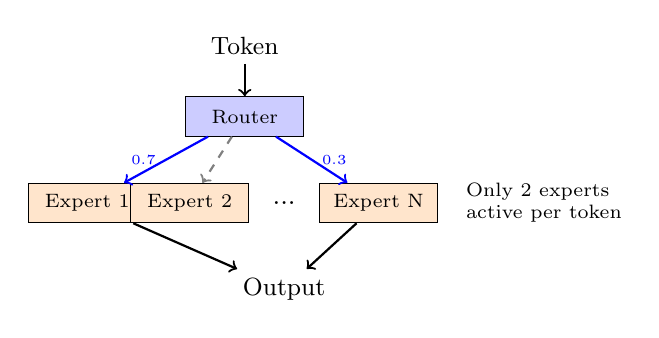
\begin{tikzpicture}[
    node distance=0.6cm,
    block/.style={rectangle, draw, minimum width=1.5cm, minimum height=0.5cm, font=\scriptsize},
    expert/.style={block, fill=orange!20},
    router/.style={block, fill=blue!20},
    arrow/.style={->, thick}
]
% Input
\node (input) {\small Token};

% Router
\node[router, below of=input, yshift=-0.3cm] (router) {Router};

% Experts
\node[expert, below of=router, xshift=-2cm, yshift=-0.5cm] (e1) {Expert 1};
\node[expert, below of=router, xshift=-0.7cm, yshift=-0.5cm] (e2) {Expert 2};
\node[below of=router, xshift=0.5cm, yshift=-0.5cm] (dots) {...};
\node[expert, below of=router, xshift=1.7cm, yshift=-0.5cm] (en) {Expert N};

% Output
\node[below of=dots, yshift=-0.5cm] (output) {\small Output};

% Arrows
\draw[arrow] (input) -- (router);
\draw[arrow, blue, thick] (router) -- (e1) node[midway, left, font=\tiny] {0.7};
\draw[arrow, gray, dashed] (router) -- (e2);
\draw[arrow, blue, thick] (router) -- (en) node[midway, right, font=\tiny] {0.3};
\draw[arrow] (e1) -- (output);
\draw[arrow] (en) -- (output);

% Annotation
\node[right of=en, xshift=1.5cm, align=left, font=\scriptsize] {Only 2 experts\\active per token};

\end{tikzpicture}
\caption{MoE: router selects which experts process each token. Most experts stay idle.}
\label{fig:moe-architecture}
\end{figure}
